\section{DevOps}
DevOps ist eine Philosophie oder Organisationsform, mit der Continuous Delivery besonders gut funktioniert. Es stellt dabei eine Kollaboration zwischen Entwicklung (Developement) und Betrieb (Operations) in den Mittelpunkt, welche in einer klassischen Organisationsform in mindestens zwei unterschiedliche Abteilungen getrennt sind. Daher beginnt DevOps bereits in den obersten Managementebenen. 
Bei der Einführung von Continuous Delivery sollten Betrieb und Entwicklung zusammenarbeiten. Jede dieser Gruppen beherrscht einen Teil von Continuous Delivery besonders gut. Der Betrieb kennt Aspekte wie Monitoring, Security oder Netzinfrastrukturen, ohne die eine Anwendung kaum sinnvoll installiert oder betrieben werden kann. Die Entwicklung hingegen kennt den Code, die Entwicklungsinfrastruktur und beispielsweise Middleware wie Application Server sehr genau. Zusammen kann eine Continuous-Delivery-Pipeline sehr einfach aufgebaut werden. Daher sollte zusammen mit Continuous Delivery auch die Einführung von DevOps (siehe Kap. 11) zumindest betrachtet werden.\\ \\
Bereits 2006 wurde bekannt, dass eines der großen IT-Unternehmen einen anderen Ansatz zur Erstellung seiner Dienste verfolgte. Die Trennung von Betrieb und Entwicklung wurde bis dato von allen IT-Organisationen verfolgt, doch zu diesem Zeitpunkt setzte Amazon bereits Teams ein, die sowohl Entwicklung als auch Betrieb abdeckten. Jedes Team ist dabei für einen bestimmten fachlichen Service zuständig. Dadurch kann jedes Team seinen Service selbst optimieren, dass er sowohl gut betrieben als auch leicht weiterentwickelt werden kann. So kann ohne weitere Abstimmung eine Erweiterung am Dienst vorgenommen werden. Auch der eingesetzte Technologie-Stack ist abhängig von der Entscheidung des Teams. Der Begriff DevOps entstand schließlich 2009 bei einer Konferenz in Belgien und setzt sich aus Development (Entwicklung) und Operations (Betrieb) zusammen, wodurch bereits der Kern des Gedanken hervorgeht: ein Zusammenwachsen der beiden Abteilungen zu einer Einheit (siehe Abbildung \ref{fig:devops}) [1]. \\
\begin{figure*}[h!]
	\centering
	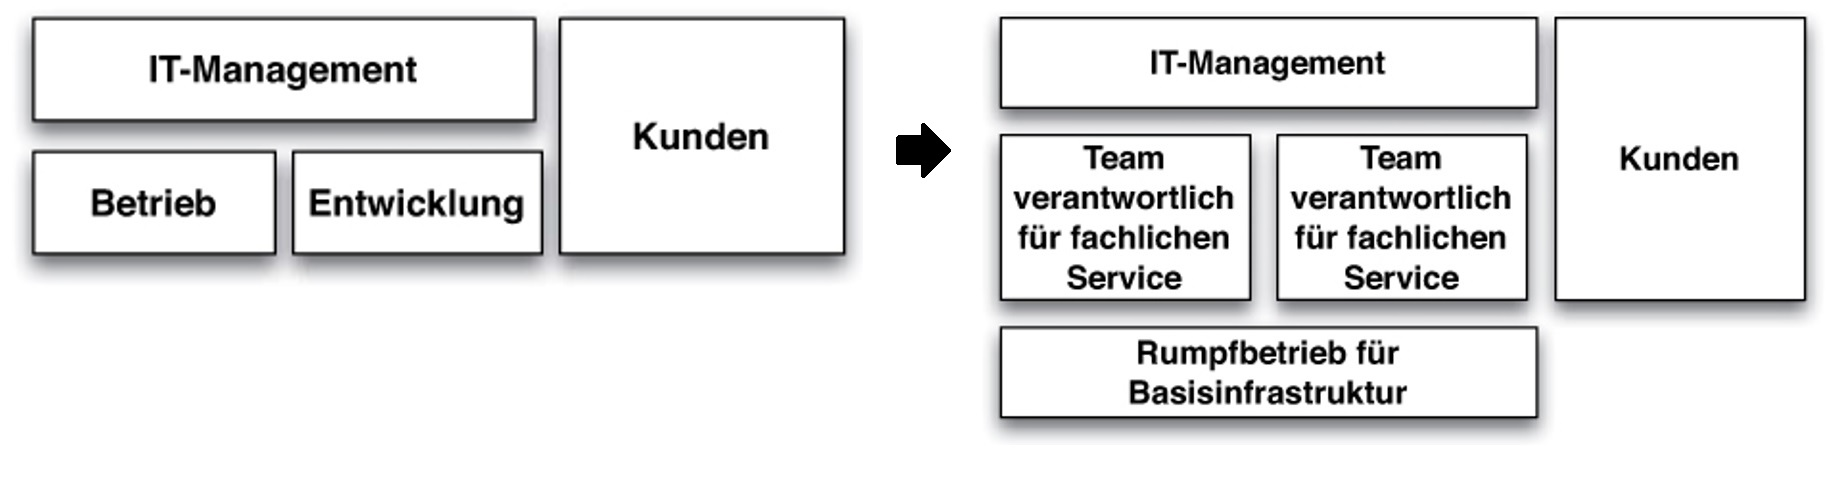
\includegraphics[width=0.8\linewidth]{images/devops}
	\caption{Wandel von klassischer Organisation zu DevOps-Teams} %Generelle
	\label{fig:devops}
\end{figure*}
\\ \\Im Kern geht es bei DevOps um Eigenverantwortung. Die Teams übernehmen die vollständige Verantwortung für eine Komponente – sowohl für den Betrieb wie auch für die Entwicklung. So müssen sich die Teams viel weniger koordinieren. Alles, was mit einer Komponente zusammenhängt, kann von einem einzigen Team bearbeitet werden. Das betrifft die Entwicklung wie auch den Betrieb und vor allem das Ausrollen in Produktion. Das erlaubt es den Teams, viel schneller zu arbeiten, Software schneller zu entwickeln und in Produktion zu bringen. [1]
Oft wird Continuous Delivery sogar mit DevOps gleichgesetzt. Das trifft aber nicht den Kern der Sache. Continuous Delivery wird zwar durch DevOps deutlich vereinfacht und ist auch eine wesentliche Praktik im DevOps-Umfeld. Aber neben Continuous Delivery gibt es noch viel mehr Bereiche, in denen DevOps als Organisationsform hilfreich ist [1]
Es ist also offensichtlich, dass DevOps weit mehr ist als nur Continuous Delivery. Es ist ein Mind Set und eine Organisationsform, die zu vielen technischen Maßnahmen führen kann, von denen Continuous Delivery nur eine ist [1].